%%%%%%%%%%%%%%%%%%%%%%%%%%%%%%%%%%%%%%%%%%%%%%%%%%%%%%%%%%%%%%%%%
%%%  Capstone Project Template that tries to save a few trees %%%
%%%  Edwin Blake 22 Aug 2013                                  %%%
%%%		1 Aug 2014 (revised)                                  %%%
%%%             10 Aug 2015                                   %%%
%%%  see also                                                 %%%
%%% http://ravirao.wordpress.com/2005/11/19/latex-tips-to-meet-publication-page-limits/
%%%%%%%%%%%%%%%%%%%%%%%%%%%%%%%%%%%%%%%%%%%%%%%%%%%%%%%%%%%%%%%%%

\documentclass[11pt,a4paper]{article}
\usepackage[htt]{hyphenat}
% Allow verbatim input to be included (for the unit tests)
\usepackage{verbatim}
\usepackage{times}
% Allows better control over headers and footers
\usepackage{fancyhdr}
% set the margins using the geometry package (which is much the easiest way of
% doing this).
\usepackage[margin=2.5cm]{geometry}
% Pictures (means you have to produce pdf output via pdflatex)
\usepackage[pdftex]{graphicx}
% Set a default path for the image files
\graphicspath{{./images/}}
% Clickable hyperlinks
\usepackage{hyperref}
% Import bib latex package
\usepackage{biblatex}
% Import the bibliography file
\addbibresource{bibliography.bib}
% Try to reduce the white space latex loves so much
\usepackage[small,compact]{titlesec}
% Reduce space around section heads and add a full stop after the number
\titlelabel{\thetitle. \quad}
% Use fancy headers
\pagestyle{fancy}
% Change name of Abstract to nothing and loose some of the excessive white
% space
\renewcommand{\abstractname}{\vskip -5mm}

\begin{document}
\title{Final Report: RoboViz Capstone Project} \date{}
\author{Boyd Kane\\KNXBOY001\\KNXBOY001@myuct.ac.za
\and Imaad Ghoor\\GHRIMA002\\GHRIMA002@myuct.ac.za
\and Jesse Sarembock\\SRMJES001\\SRMJES001@myuct.ac.za}

%  Set the headers via fancyhdr package
% Short title for running head
\lhead{RoboViz Final Report}
\chead{}
\lfoot{}
% add page number as centre footer.
\cfoot{\thepage}
\rfoot{}
% Don't want horizontal line under header
\renewcommand{\headrulewidth}{0.0pt}

\maketitle
% First page is plain style headings and footers (ie just the page number as
% footer).
\thispagestyle{plain}

\begin{abstract}
% First you should have an executive summary (or abstract) just a single
% paragraph saying what the results of the project are (at most 200
% words).
    The RoboViz Project extends an existing open source genetic evolution
    platform (RoboGen) to permit the visualisation of multiple robots, called a
    swarm. The RoboViz Project accepts multiple parameter to fine-tune the
    simulation of the swarm, and adheres to OOP best practices.
\end{abstract}

% We expect a report of about 3500-4000 words, written single spaced, with a font
% size of at least 11 pts.  Use at least a 2.5 cm margin on all sides of the
% pages.
%
% No blank lines between paragraphs except to get figures and their captions to
% position properly.
%
% Depending on how many diagrams you use (more is better) the report will be
% between 7 and 10 pages long. Your appendices (e.g., user manual, test results,
% which are needed) are not included in these limits.
%
% You must had-in an Adobe Acrobat file for your report (i.e., pdf
% file).
% You should begin your write-up with an overview and then drill down
% into the details of what you produced. Your report should cover the
% following sections (Sections \ref{s:introduction} --
% \ref{s:conclusion}).
%
% Some notes about code formatting
% - Each method should start with a brief description of its
%   function.
% - Use indentation to display the structure within a method.
% - Comments should be used extensively. They are best used to
%   describe logical blocks of code rather than individual
%   statements. Line-by-line comments have the drawbacks of not
%   providing any overview and of decreasing readability.
% - Meaningful identifiers should be chosen.
% - Output should be pleasingly formatted and easy to read.
%
% You do, of course, have the option to call in any of your
% favourite packages for setting maths, graphics, computer listings,
% etc.

\tableofcontents
\section{Introduction}
\label{s:introduction}
% Your introduction provides the context for the project and should
% contain the statement of the scope of the project (which may have
% changed since you first wrote it). Someone reading your introduction
% must have clear idea of what the system is intended for. If you think
% there is something special about the kind of problem you tackled that
% your reader needs to know up front then this is where you say it.
%
% If you need any survey of other work (you probably don't) then put it
% towards the end of the introduction and give suitable references. A
% case where this is needed is if your project builds on someone else's
% project or some published algorithm.
%
% Discuss your approach to solving the problem. Please give a short
% overview of the software engineering methods you used (e.g.,
% traditional analysis followed by design and implementation -- typically
% the case if you did an evolutionary prototype, or a more agile
% approach where you had a cyclical development process).

This project - RoboViz - involves extending an existing visualiser
\cite{robogen} to enable the visualisation of multiple of multiple robots
simultaneously.  Robogen allows researchers to define a robot structure and
then make use of genetic algorithms (paired with a fitness function) to evolve
robots that that gradually perform better (as a measured by the relevant
fitness function) as more generations of robots are simulated.

After a set number of generations, the final robot can also be visualised,
although currently the software only allows for the visualisation of a single
robot. The software also generates STL files which describe the 3D body parts
of the robot, such that a 3D printer can take those files and 3D print the body
components of the evolved robot. INO files are also generated, which can be
loaded onto the Arduino platform and define the robot’s ‘brain’ as a software
defined artificial neural network which was evolved by the genetic algorithm.

This project involves modifying the source code of the RoboGen software and
proving that the modifications are efficient enough for at least 3 (but
preferably more) robots to be simulated at once.

An agile software development approach was taken to develop this project. The
project team has worked over WhatsApp and MS Teams, informing each other on
their work and designating tasks from there. Time was spent on creating
functional code to implement a swarm of robots and testing that code before
adding more functionality. The team has had frequent meetings with project
stakeholders, receiving feedback directly from the stakeholders while
developing the project. Throughout development, there have been a significant
number of changes needed as development progressed and these were added to the
project plan over time.

A vertical prototype was chosen for this project since it focuses on
implementing a specific feature - swarm of robots in the visualiser - this was
the most appropriate prototype as it tests key components during early stages
of the project to check key functions.

The existing RoboGen \cite{robogen} lacked any sort of automated documentation,
and so the Doxygen documentation tool \cite{doxygen} was also added to the
project, in order to automatically generate documentation from the source code
of the project.  Following this, the source code was annotated with well
formatted comments that could be parsed by Doxygen. The html documentation can
be found in \texttt{src/docs/html/index.html} but it is not kept under version
control. The Doxygen documentation, as well as the final report, can be
generated with the following command:

\begin{verbatim}
cd roboviz/src/docs && ./build_docs.sh
\end{verbatim}

\section{Requirements Captured}

\subsection{Functional Requirements}
The final project must be able to visualise at least 3 robots simultaneously.
The morphology and neural network defining these robots must be defined in a
file as per existing RoboGen guidelines for defining robots (as either
\texttt{json} or specially formatted \texttt{txt} files). The user must be able
to zoom in and out of the simulation, as well as pan across to view different
parts of the simulation with more clarity. The user must also be able to pause
and unpause the simulation.

\subsection{Non-functional Requirements}
The user should be able to interact smoothly with the simulation once started.
That is, the simulation should not close before the specified simulation
duration is over. The simulation should start within 2 minutes of running the
\texttt{robogen-file-viewer} executable. On an adequately powerful machine, the
swarm should be simulated at more than 15 frames per second.

\subsection{Usability Requirements}
While the simulation is running, console based output should inform the user of
the details of the simulation, for example, when robots are added to the swarm
or which configuration files are being read. This output should be well
formatted and provide information on various levels useful for finding
problems, warning the user about potential issues, and if an error occurs,
providing the user with sufficient information to solve the error.

% Discuss the major analysis artefacts that you produced. We will expect
% you to produce at least one overall description of the architecture
% used in your system as a diagram, either here or below (see Section
% \ref{s:design-overview}). You may also want to include an analysis
% class hierarchy diagram.

% TODO Discuss the 'major analysis artefacts'
\subsection{Use Case Narratives}
See Figure \ref{fig:use-case-diagram} for the Use Case Diagram.
\begin{figure}[htpb]
    \centering
    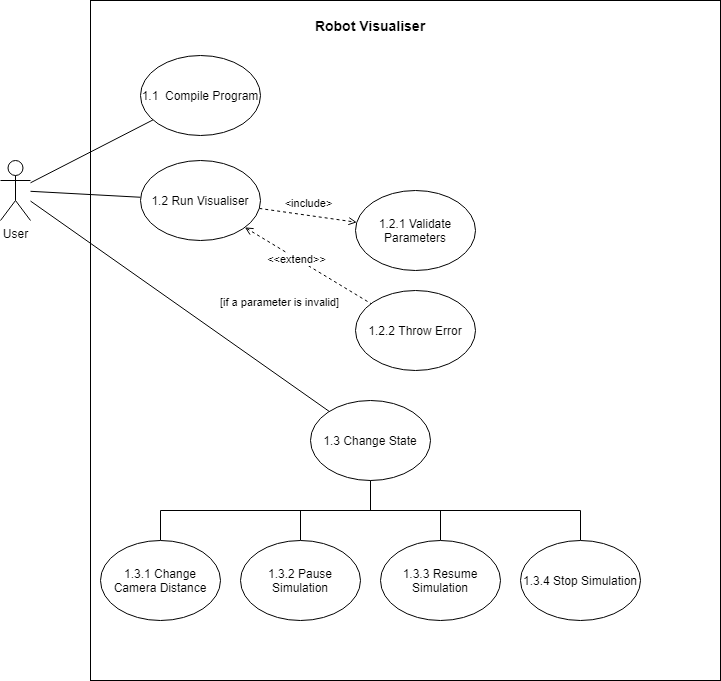
\includegraphics[width=0.5\textwidth]{2}
    \caption{Use Case Diagram}
    \label{fig:use-case-diagram}
\end{figure}
\subsubsection{Start Simulation of the Swarm. Actor: User}
\paragraph{Primary Path:} The user runs the program and is prompted to enter
the name of a robot file and a configuration file (which includes how many
robots to simulate in the swarm).  The program loads a new window that is the
visualiser, and displays the specified number of robots performing their tasks
from the same robot file.  While the simulation is running, the user may pause
the simulation and zoom into the area where the robots are performing for a
closer view.

\paragraph{Alternative Path:} If the robot file entered is incorrectly
formatted or does not exist then the program will throw an error and return the
command line help page.

\subsubsection{ Run Visualiser. Actor: User}
\paragraph{Primary Path:} The user starts the visualiser, after that, the user
needs to enter 2 parameters, location of the file that defines the robot and
the location of the file that defines requirements and configurations for the
file viewer. Should one of the parameters entered be invalid or non-existent,
an exception will be thrown, requiring the user to enter those parameters
again.

\subsubsection{ View Simulation. Actor: User}
\paragraph{Primary Path:} Once the simulation displays the robots performing
their tasks in the run-time environment. The user may change the state of the
view, by pausing,resuming and stopping the simulation. The user may also zoom
in closer to the robots or zoom further away. The simulation will stop once the
time limit specified in the configuration file has passed.

\section{Design Overview}
\label{s:design-overview}
% The next section is an overview of your design. The system design has
% to be justified in terms of the expected behaviour of the final
% product.
%
% If you produced a design class diagram put it here.
% \begin{figure}[h!]
%   \center{\includegraphics[scale=0.8]{architecture.png}}
%   \caption{An architecture diagram. Caption to go below figure}
%   \label{fig:architecture}
% \end{figure}
%
% You must present the overall architecture of the system together with
% an architecture diagram. You may choose what kind of diagram best
% suits your project but we would expect a layered architecture diagram
% (see Figure \ref{fig:architecture}) unless there is a good reason for
% some other kind of diagram. It need not be a formal UML diagram as
% long as it conveys all the necessary information clearly.
%
% You should then (in subsections) cover the algorithms and the data
% organisation used and why they were considered the best.

Given that the project authors were extending the existing RoboGen
\cite{robogen} code base, changing some existing aspects of the existing
software was considered out of scope due to time constraints and for existing
RoboGen users to easily learn to use the RoboViz project.


\subsection{Layered Architecture Diagram}
% TODO Add layered architecture diagram to present the overall architecture of
% the system.

\subsection{Swarm Class}
The starting point of our design process was the Swarm Class.
This is a class that acts as a container of Robot objects. By implementing such a class,
we were able to store multiple instances of Robot objects and then alter the codebase to
reference Robot objects through the Swarm class, which was integral to obtaining swarm functionality.

\subsection{SwarmPositionsConfig Class}

This class is responsible for initializing the position of each robot in the swarm in the environment.
It also creates a message containing these coordinates.

\subsection{Analysis Class Diagram}
See the Analysis Class Diagram in Figure \ref{fig:analysis-class-diagram}

\begin{figure}[htpb]
    \centering
    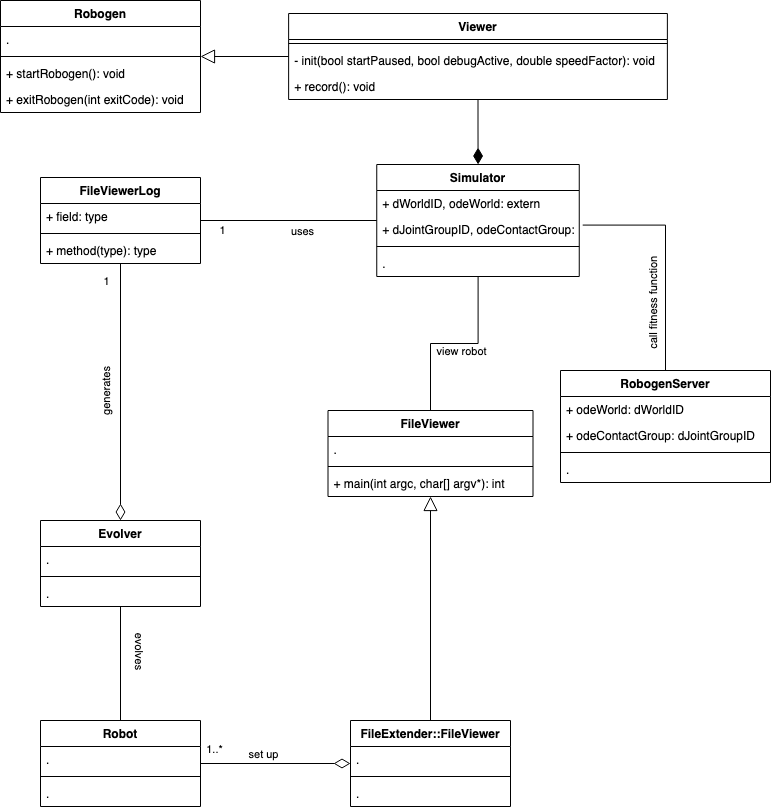
\includegraphics[width=0.5\textwidth]{1}
    \caption{Analysis Class diagram}
    \label{fig:analysis-class-diagram}
\end{figure}

\section{Implementation}
% Now we get to the details.
% - Describe your data structures and be sure to illustrate them with a
%     diagram.
% - If your user interface was a key feature describe how that was
%     implemented.
% - Discuss the function of the most significant methods in each class.
%     This may well require flowcharts, or sequence diagrams, in some cases.
% - Any special relationship between the classes (e.g. friends) and why
%     they exist.
% - A description of any special programming techniques or libraries
%     used.


\subsection{Overview}
The changes made to the existing project will be covered in the same order as
they are encountered when a user runs the final executable.

The \texttt{robogen-file-viewer} is the executable used to run the simulation
such that the swarm can be watched in real time. This executable had to be
modified to read in some additional parameters (for example: \texttt{swarmSize}
, \texttt{swarmPositions}) via configuration files, and then to store those
parameters in the existing \texttt{RobogenConfig} object along with the other
configurations. Since the positions of the robots in the swarm has to be
specified in a separate file, this also required creating a new file
configuration reader (\texttt{SwarmPositionsConfig}) to parse the swarm
positions. This file was created to be similar to the existing
\texttt{ObstaclesConfig} and \texttt{LightSourcesConfig} objects, and was
integrated to the existing \texttt{ConfigurationReader}.

Once the configurations for a swarm are read in, error checking is done on
those configurations and the program exits if the user requests an invalid
combination of options (for example, a negative \texttt{swarmSize}).
At this point various logging objects are initialised, and these were modified
to log the details of every robot in the swarm.

At this stage the robots are initialised, with source files and swarm size
specified in the above mentioned configuration files. Each robot's sensors,
actuators, and its neural network are also initialised here. This can take some
time, and so sufficient log output is printed to keep the user informed.

Now that everything is initialised, the main loop of the simulation begins. The
simulation can run once (as is the case for a simple visualisation) or it can
run multiple times (as is the case for when a population of swarms are being
evaluated by the evolver. There are various protections in place to ensure the
swarm is not taking advantage of errors in the physics simulation, which were
developed to handle more than one robot. Additionally the evaluation of the
individual robot's neural networks had to be extended to work for more than
just one robot.

On completion of the simulation, the memory required by the dynamics engine
\cite{ODE} and the RoboViz swarm is freed.

\subsection{Data Structures Used}
\subsubsection{Swarm Class}
The Swarm class ( \texttt{src/Swarm} ) is the internal representation of a
collection of robots. The members of the swarm are assumed to be attempting to
cooperate with one another, and receive a single fitness score at the end of a
scenario.

\subsubsection{RobogenConfig Class}
The simulator is designed to be flexible, and as such requires a lot of
configuration parameters to be specified. These configurations are stored in
the \texttt{RobogenConfig} object, often named \texttt{config} in the code
base. However, the \texttt{RobogenConfig} object is only responsible for storing the
well formatted and easily accessible parameters. The responsibility of parsing
those parameters is handed to the \texttt{ConfigurationReader} class:

\subsubsection{ConfigurationReader Class}
The configuration parameters for the scenario (like the type and size of
terrain, the starting positions of the robot(s), the fitness function to use)
are parsed by the \texttt{ConfigurationReader}. Some of the parameters are
specified directly in the configuration file as key-value pairs separated by an
equals \texttt{=} symbol, while other parameters have values referencing
relative file paths where a list of values can be found. These external
parameters are parsed separately by different config classes (for example,
\texttt{ObstaclesConfig}, \texttt{LightSourcesConfig}, and
\texttt{SwarmPositionsConfig}.

\subsubsection{SwarmPositionsConfig}
The x,y,z locations of the individual members of the swarm can be specified in
a separate file, and this file is parsed by the \texttt{SwarmPositionsConfig}
object. The object is instantiated as a member of the
\texttt{ConfigurationReader}, and these configurations can later be accessed
during simulations.

\subsubsection{Scenario}
A scenario is the combination of a swarm in rigid body simulation with a
fitness function. When a scenario is initialised, the swarm is instantiated
into the task environment, and when the simulation starts the swarm will be
monitored by the scenario so that it's fitness can be calculated. A custom
fitness function can be defined by creating a javascript file with the
appropriate callbacks, or one of \texttt{racing} (fitness is proportional to
average distance from the starting position) or \texttt{chasing} (fitness is
inversely proportional to distance from the nearest moving light source) can be
chosen. These fitness functions are defined in the various files found in
\texttt{src/scenario/}

\subsubsection{FileViewer Class}
The \texttt{FileViewer} is the command line entry point for starting a
simulation. It takes in two command line arguments (the path of the file
defining the robots, and the path of the configuration file), parses those
arguments using \texttt{boost} program options \cite{boost}. This is the file
that becomes the executable used to start the simulator for the purpose of
viewing a swarm.

\subsubsection{IViewer Class}
This is an interface defining common functionality for classes wishing to view
the current state of a simulation. For example, the simulation can be viewed in
the web browser or on desktop.

\subsubsection{Simulator}
The \texttt{Simulator} has a single (overloaded) method,
\texttt{runSimulations} which receives a scenario, a RobogenConfig, and
optionally a viewer. This method then initialises the viewer (if applicable),
each robot in the swarm, the rigid body simulator, ODE, and sets up the
scenario in anticipation of calculating the fitness of the swarm. The
simulation is then started up, and run for a duration specified in the
\texttt{RobogenConfig} object. This duration from starting the simulation in
the world until the simulation is destroyed is called a trial. The simulator
can be specified to perform multiple trials, or just one.

When the specified number of trials has been completed, the dynamics engine is
closed, and all resources are cleaned up.

\subsubsection{robogen.proto}
Most objects in the Robogen project can be serialised into Google Protocol Buffer
Messages \cite{protobuf}, which provide a language and platform neutral method
for serialising structured data, similar to XML but faster and simpler. The
file \texttt{robogen.proto} contains definitions of the structure of the data,
and was extended to allow the swarm class to be serialised.


\subsection{Overview of the User Interface}
% TODO Brief overview of the user interface (don't need to go in depth, it
% wasn't a major part of the system)
\subsection{Most Significant Methods of Each Class}
Note that, due to the immense size of the existing code base, only classes
to which substantial changes were made are included in this subsection.

\subsubsection{Configuration Reader and RobogenConfig}
The configuration reader (\texttt{src/config/ConfigurationReader.cpp}) is in
responsible for receiving a file name with configurations and parsing them into
a \texttt{RobogenConfig} object (\texttt{src/config/RobogenConfig.h}). The
configuration reader has one primary method \texttt{parseConfigurationFile}
which receives the file name and returns a properly formatted
\texttt{RobogenConfig} object. This method and the header file for the
\texttt{RobogenConfig} object had to be extensively reworked to allow for
specification of the swarm size, the gathering zone size, the gathering zone
position, the swarm positions, the file containing the swarm positions, and the
file containing the resources configuration.

The obstacles, light sources, and swarm start positions are all specified in
separate files, and so there are separate methods to parse those files and
return pointers to the appropriately named configuration objects. The methods
are \texttt{parseObstaclesFile}, \texttt{parseStartPositionFile}, and
\texttt{parseLightSourcesFile}.

\subsubsection{Simulator}
The simulator (\texttt{src/Simulator.cpp}) contains just one (overloaded)
method, \texttt{runSimulations}. This made testing this class exceedingly
difficult, and highlighted the importance of not having `god classes' as
mentioned in our Advanced Software Development lectures. This methods receives a
scenario, a configuration, a swarm, and optionally a viewing window. It is in
charge of running a certain number of trials in a scenario. A trial is one
iteration of the swarm being initialised and then started to complete it's
goal. A scenario is the collection of variables that defines the swarms
surroundings and environment. The simulation can either be done headless
(without being rendered to a screen for a person to view it) or it can be done
with a viewer, so that a person can view the simulation as it is running.

Since this method was so tightly coupled with the \texttt{Robot} class, it
required a lot of work to refactor so that it would work properly and
efficiently with the new \texttt{Swarm} class.


\subsubsection{File Viewer}
The File Viewer (\texttt{src/viewer/FileViewer.cpp}) has two components which
are handled by the \texttt{C++} preprocessor, only the second of which was
modified for this project. The first component takes care of \texttt{emscripten}
content which is used for when the program is being displayed in a web browser
via JavaScript, and the second component takes care of the case when the
program is being run on the desktop via \texttt{C++}.

Despite the misleading name, this is the main executable which is run after
compilation in order to view a simulation run, and so has a standard
\texttt{C++} \texttt{int main()} method, along with some minor utility methods
to print the usage information for the command line interface (\texttt{void
printUsage()}), another to print the help information for the configuration
files (\texttt{void printHelp()}), and some other less important utility
methods.

The main method parses the commandline arguments, ensures they are properly
formatted, and then passes the configuration file to the
\texttt{ConfigurationReader}. There is a lot of error checking to be done for
the various commandline arguments, but if they are all properly specified and
there are no illegal combinations (like requesting to record the simulation
without also specifying that the simulation should be visualised) then a swarm
is created from the input file specified via a commandline argument and the
scenario, the logger, and optionally the viewer are all initialised.

Following this, the simulation is started via a method call to
\texttt{runSimulations}. When the simulation has finished and returned, the
fitness of the scenario is calculated and displayed to the user. After some
clean up, the method ends and the program terminates.

\subsubsection{Viewer}
The viewer (\texttt{src/viewer/Viewer.cpp}) is responsible for rendering a
scene containing a swarm, obstacles, light sources, and the terrain. This is
largely a wrapper around OpenSceneGraph, which is where the actual rendering
and window management takes place. The file's primary method is
\texttt{configureScene} which will take a scenario and a collection of models
defining the body parts of the swarm, and link them all together. It will then
render the terrain, the obstacles, and the light sources, and create the camera
in the scene so that the user can see how the simulation is progressing.

The other methods in this class are largely utility methods, used to check or
modify the state of the viewer.

\subsubsection{Obstacles, Swarm Positions, and Light Sources Config}
There are three types of objects which have configuration parameters specified
not in the main configuration file, but in separate files which the main
configuration file contains references to. These are the
\texttt{src/config/ObstaclesConfig.h}, the \texttt{src/config/LightSourcesConfig.h}
and the \texttt{src/config/SwarmPositionsConfig.h}. They are all structured
similarly, with methods to get the relevant configuration parameters (like
\texttt{getCoordinates()} or \texttt{getDensities()}, etc) and a
\texttt{serialize()} method which converts the configuration object into a
Google Protocol Buffer Message.


\subsubsection{Swarm Class}
The \texttt{getRobot(int i)} method returns a pointer to the i-th robot in the swarm.
The \texttt{addRobot(boost::shared\_ptr<Robot> robot)} adds a robot to the swarm, by
pushing it to the back of the vector of robots.

\subsubsection{RobogenCollision Class}

The \texttt{prune()} method resets the environment and all of the robots to their
initial states.  The \texttt{getSwarm()} method returns a pointer to the swarm of
robots.  The Scenario constructor sets up the environment for a given scenario
by initializing objects such as \texttt{lightSources,} obstacles, and robots.

\subsubsection{ChasingScenario Class}

The \texttt{setupSimulation()} method initializes the distances in the distances vector
to 0.  This is the first step to calculating the fitness of the swarm.  The
\texttt{afterSimulationStep()} method evaluates the distance of each robot from its
corresponding light source at the end of the current trial, and updates this
value in the distances vector.  The \texttt{endSimulation()} method increments the trial
counter and resets the starting positions for the next trial.  The \texttt{getFitness()}
method calculates the fitness of the swarm for the chasing scenario by
calculating the average distance from a robot to its corresponding light
source.

\subsubsection{JSScenario Class}
The \texttt{printRobotPosition()} method prints out the position of the robots at the
current trial.

\subsubsection{QScriptScenario Class}
The \texttt{getFitness()} method calculates the fitness of the swarm for the
\texttt{QScriptScenario} case.

\subsubsection{RacingScenario Class}
The \texttt{endSimulation()} method evaluates the distance of each robot from its
starting position and updates this value in the distances vector.  The
\texttt{getFitness()} method evaluates the fitness of the swarm for the Racing Scenario
by calculating the average distance that each robot has moved from its starting
position.

\subsubsection{WebGLLogger Class}
The \texttt{generateBodyCollection(int s)} method creates a \texttt{BodyDescriptor} struct for
every body part of robot s and adds this to a bodies vector. The bodies vector
of each robot is then added to the \texttt{vectorOfBodies,} which holds bodies vectors
for each robot in the swarm.

\subsection{Special Relationships between Classes}
Due to its size, the existing Robogen code base is highly connected and has
many relationships between classes. This subsection only attempts to describe
those relationships that are essential to the RoboViz project and those
relationships which were introduced by the RoboViz project.

A \texttt{Swarm} is defined as a collection of \texttt{Robot} objects which
themselves are constructed from various classes which define the morphology of
the robot, the neural network controlling the robot, and the simplified
physical representation of the robot used by the simulator for physics
calculations.

A Swarm is created to complete some user-defined task in an environment. The
Scenario class is that environment combined with parameters defining the
terrain, obstacles, light sources, the method of evaluating how well the swarm
accomplished its task, and various physics engine parameters. Since the physics
engine is not entirely deterministic by design, a scenario can be run multiple
times (called trials), resulting in a fitness value for each trial. A
collection of trials being run from start to finish is handled by the Simulator
class.

There is also the option for a human to view the simulation as it progresses.
This is done by providing an optional Viewer to the scenario, which will be
initialised and destroyed in line with the life cycle of the simulation.

The evolution engine was not changed and so will not be described in this
outline.



\section{Program Validation and Verification}
\label{s:progr-valid-verif}
% Tell us how you tested the system and why you believe it works.
% Describe the Quality Management Plan for your project, that is,
% software testing plan. The plan should indicate the types of testing
% that was performed and detail how they were done. This must include
% the reasons on why the chosen testing protocol was considered
% effective.
%
% Create a table that summarizes the testing plan (see Table
% \ref{tab:test-plan}).
%
% Describe all the steps taken to validate the correctness of the
% program.
%
% If you had user tests then say what you did and what the results
% were. Describe why these test data were chosen (what test conditions
% the data was testing).  Table \ref{tab:tests} provides an example of
% the sorts of results we are looking for. The full detail of the test
% runs should be appended to the report.

\subsection{How the system was tested}
The testing frameworks \texttt{GoogleTest} and \texttt{GoogleMock} were used to
run tests on the code base, and these tests were integrated with the existing
\texttt{CMake} files so that tests are compiled automatically and can be run
via the command \texttt{ctest}. Testing covered some aspects of the existing
code base but due to it's size (164 thousand source lines of code) the primary
focus was on the additions made by the RoboViz project in the \texttt{Swarm}
and \texttt{ConfigurationReader} classes. These test are run automatically when
the rest of the code base is compiled, so that no changes can get through which
break existing functionality.


\subsection{How we know the system works}
The RoboViz team has confidence that the existing system works due to the tests
that have been put in place to assure us of this. If something were incorrect,
the tests would pick it up automatically. Since the test run automatically,
there is no scope for human error or judgement which can sometimes cause errors
to creep in.

\subsection{Type of testing, and method of test execution}
The existing code base was not structured to allow for easy testing. The levels
of coupling between different objects was very high and there exist many
methods which have a large number of side effects, reducing the atomicity of
any tests that would be run on them. The focus of the testing was on unit
tests, specifically for the additions to the code base which were made by the
RoboViz team. These unit tests were written using the \texttt{GoogleTest} testing
framework, and were integrated with \texttt{CMake} so that they would compile
and run automatically.

\subsection{Justification of the chosen testing plan}
The testing plan was chosen to be effective yet efficient, given that complete
test coverage was infeasible due to the size of the project and the duration of
time given to complete the project. The existing test were written to cover the
most likely of errors and the most fatal of errors of the existing code base,
as well as to cover the newly written code so that problems have the greatest
likelihood of causing a test to fail.

\subsection{Use of mock data in the tests}
Mock data was used in the form of valid or invalid input files, stored in
\texttt{examples/test\_cases/} as files named like the tests that use them.
These data provide common mistakes made when specifying the input files, and
the tests are written to check against these common errors.

\subsection{Full detail of the test runs}
The full details of the test runs can be found in the Appendix, section
\ref{s:full-test-runs}.


\subsection{Usefulness of the system based on the unit tests}
The system is considered by the authors to be more useful and more error-save
(thereby more usable) than the original project for various reasons. Firstly,
the addition of the tests and the setup of the testing framework means that any
problems in the future will be found by the existing tests, and adding new unit
tests to cover future expansions are made easier. Secondly, the extensive
documentation (in the code base in the form of Doxygen comments, in the
\texttt{CONTRIBUTING} file, and in the commandline-help that gets printed when
a user specifies the wrong arguments) mean that future users will easily be
able to get started, as we have extensively logged our troubles with the code
base (and the solutions to those troubles) via these means.

\begin{table}[h!]
    \centering
    \caption{Summary Testing Plan}
    \begin{tabular}[t]{|p{8cm}|p{7cm}|} \hline
        \textbf{Process} & \textbf{Technique} \\
        \hline 1. Class Testing: test methods and state behaviour of classes
                         & Via class-by-class tests in the appropriately named
                         test files\\
        \hline 2. Integration Testing: test the interaction of sets of classes
                            & Due to the highly-coupled design of the existing
                            code base and the extensive side effects that occur when
                            classes interact, integration testing had to be
                            covered by the new unit tests.\\
        \hline 3. Validation Testing: test whether customer requirements are
        satisfied
                            & The client expressed satisfaction with the
                            prototype and agreed with our plans for further
                            development after the prototype. The client's
                            requirements were manually considered and found to
                            be satisfied.\\
        \hline 4. System Testing: test the behaviour of the system as part of a
        larger environment
                            &  The testing framework was executed on different
                            environments, resulting in the stability of the
                            platform in different situations being established.\\
        \hline
    \end{tabular}
    \label{tab:test-plan}
\end{table}

\begin{table}[h!]
    \centering
    \caption{Tests used to ensure correct functioning of the code base.}
    \begin{tabular}[t]{|p{4cm}|p{4cm}|p{5cm}|} \hline
        \textbf{Test File Name} & \textbf{Test Name} & \textbf{Test Description} \\
        \hline  SwarmTest & OnInitThenSizeIsZero & Check swarm size is zero on
        initialisation. \\
        \hline  SwarmTest & OnAddRobot ThenSizeIncrements & Check the swarm size
        variable is incremented when a robot is added to the swarm\\
        \hline  SwarmTest & OnAddRobot ThenReturnsCorrectRobot & Check when a
        new robot is added to the swarm, then that robot is returned by the
        appropriate \texttt{getRobot(i)} call.\\
        \hline  ConfigurationReaderTest & DisplaysHelp & Check the
        ConfigurationReader will display help to the user when they input
        invalid commandline arguments.\\
        \hline  ConfigurationReaderTest & ParsesSwarmSize & Check the
        ConfigurationReader correctly reads in and parses the swarm size from
        the configuration file.\\
        \hline  ConfigurationReaderTest & ParsesRacingScenario & Check the
        ConfigurationReader correctly reads in and parses the racing scenario from
        the configuration file.\\
        \hline  ConfigurationReaderTest & ParsesChasingScenario & Check the
        ConfigurationReader correctly reads in and parses the chasing scenario from
        the configuration file. \\
        \hline  ConfigurationReaderTest & ReadsSwarmPosFile & Check the
        ConfigurationReader correctly reads in and parses the swarm position
        file from the configuration file. \\
        \hline  ConfigurationReaderTest & ThrowsOnBadSwarmSize & Check the
        ConfigurationReader throws an error when a bad swarm size and
        swarmPositionFile combination is used in the configuration file. \\
        \hline  ConfigurationReaderTest & ParsesGatheringZone & Check the
        ConfigurationReader correctly reads in and parses the gathering zone
        file from the configuration file. \\
        \hline  ConfigurationReaderTest & ParsesGatheringZonePos & Check the
        ConfigurationReader correctly reads in and parses the gathering zone
        position from the configuration file. \\
        \hline  ConfigurationReaderTest & ParsesGatheringZoneSize & Check the
        ConfigurationReader correctly reads in and parses the gathering zone
        size from the configuration file. \\
        \hline
    \end{tabular}
    \label{tab:tests}
\end{table}
% Follow your table of results with a discussions of them highlighting
% how useful and usable your system is for its intended purpose.

\section{Group Contributions}
\label{s:group-contributions}

\subsection{Boyd Kane - KNXBOY001}
Boyd made changes to the code base, the final report, and was in charge of
rebasing the feature git branches onto the master branch. Boyd set up the
Doxygen documentation system and added properly formatted documentation comments
to the majority of the code base. Boyd set up the GoogleTest testing framework
and wrote the unit tests contained in \texttt{SwarmTest.cpp} and
\texttt{ConfigurationReaderTest.cpp}. Boyd changed the Google Protocol Buffer
definitions to handle the new Swarm object, and added code to allow the
ConfigurationReader to parse the new parameters required by the project brief
that did not exist in the original project. Boyd changed the
\texttt{Simulator} to accept a swarm instead of a collection of robots. Boyd
changed the \texttt{Scenario} initialisation to accept and initialise a swarm
of robots, and to handle the edge cases arising from that. Boyd standardised
the console log messages to have a common format, and increased the amount of
output so that the program would be more helpful to the user. Boyd changed the
\texttt{FileViewer} and created the \texttt{SwarmPositionsConfig} so that a
separate file containing a list of swarm starting positions can be specified.
Boyd started the generation of the \LaTeX report and oversaw the changes made
to it.

\subsection{Imaad Ghoor - ABCXYZ001}
TODO [imaad]


\subsection{Jesse Sarembock - ABCXYZ001}
TODO [jesse]

\section{Conclusion}
\label{s:conclusion}
% Your report must have a clear conclusion where you revisit the aims
% set out in the beginning and discuss how well you met them. Did you
% achieve the objective of creating a well-structured, modular, and
% robust system?  Please summarize the design features and test results
% that show this.
This project aimed to convert the existing code base of the RoboGen project
into a form that would allow the visualisation of a collection of robots,
called a swarm. This objective was achieved on time and as per schedule. The
project satisfies the client's primary requirements and has extensive
documentation with which the client can modify the project according to their
future needs.

One large difficulty with modifying a large existing code base like RoboGen is
that there are many places which are (unfortunately) not well-structured and
there is not enough scope to refactor the entire project. However, where
possible we have restructured the code base to better adhere to the principals
we learnt in Advanced Software Development, while still conforming with the
code style of the existing project.

\section{Limitations}
The major limitation for this project was the lack of documentation for the
pre-existing code base. Personal problems included the June exams being
postponed to a week before the (original) final hand-in, and the template-style
rubrics not applying well to our project. Due to the structure of the initial
hand ins, the full scope of the project only became apparent 4 weeks into
`starting' the project, when we finished with creating UML diagrams and started
having to edit the code base. By this time it was apparent that the full
requirements which included:

\begin{itemize}
    \item Multi-threading the physics and initialisation computations.
    \item Creating new resource blocks to exist in the world.
    \item Creating a gathering zone in the world.
    \item Rewriting the code base to use Swarms instead of robots.
\end{itemize}

Would require far more than 4 weeks of work which coincided with the 4 week
build up to exams.

\section{Bibliography}
\printbibliography

\appendix
\section{User Manual}
\label{s:user-manual}
% Your system must have a user manual. Append this to your report (make
% it Appendix A) or bind it separately if it is big. If your system is
% interactive and has a good user interface with context dependent help
% then this can be just a cheat sheet. Discuss the level at which your
% user manual is to be pitched with your client. If your system is to be
% extended then you might want to include a technical API manual.

\subsection{Introduction}
\label{s:introduction}

The purpose of the modified version of RoboViz is to enable the visualisation
of multiple robots in the task environment, as opposed to a single robot. The
number of robots that can be held in a swarm depends on how powerful the system
that is running it.

\subsection{Definitions}
\label{s:definitions}

Robot File - A file that defines a robot and its composition.

Configuration File - File that defines the behaviour of the robots when being
visualised.

Robot FileViewer or Visualiser - The window where the user will be able to view
the robots performing.

\subsection{Installation}
\label{s:installation}
Note that the installation only works for the Linux kernel. Although there are
instructions for MacOS, they do not work and a virtual machine is required if
you are not running Linux.

\begin{enumerate}
    \item There are several prerequisites. You can install them with:

    \texttt{sudo apt-get install libboost-all-dev zlib1g zlib1g-dev libprotobuf-dev}
    \texttt{protobuf-compiler gnuplot libopenscenegraph-dev cmake build-essential libtool}
    \texttt{automake libjansson-dev git libpng-dev}
    \item To clone the roboviz git repository, navigate to the directory where
        you want to store the repository and then run the command:

        \texttt{git clone https://gitlab.cs.uct.ac.za/csc3-capstone-project/roboviz.git}
    \item You will also need to install the Open Dynamics Engine via wget. This
        should be in the same parent directory as roboviz:

        \texttt{wget "https://bitbucket.org/odedevs/ode/downloads/ode-0.16.2.tar.gz"}
        \texttt{tar -zxvf ode-0.16.2.tar.gz}

    \item You will need to configure ODE to use double precision:

        \texttt{cd ode-0.16.2}
        \texttt{./bootstrap}
        \texttt{./configure --enable-double-precision --with-cylinder-cylinder=libccd}
        \texttt{sudo make install -j}
    \item Now that the dependencies are ready, change directory into the
        roboviz project folder:

        \texttt{cd ../roboviz}
    \item The build system used by RoboViz is CMake, and the unit tests are
        automatically compiled. Compile the project with:

        \texttt{cd build \&\& rm -rf *}
        \texttt{cmake -DCMAKE\_BUILD\_TYPE=Release -G"Unix Makefiles" ../src}
        \texttt{time make -j2}
        \texttt{cp -r ../models ./}

    \item  Run the tests from the build folder with:
        \texttt{ctest --verbose}

    \item Still from the build folder, the file viewer can be executed with:

        \texttt{./robogen-file-viewer ../examples/sindiso\_single.json }
        \texttt{        ../examples/sindiso\_conf.txt --debug}
    \item And that's it!
\end{enumerate}

You can run different simulations by editing the file
\texttt{examples/sindiso\_conf.txt}. More details about contributing to the
project can be found in \texttt{CONTRIBUTING.md}. Commandline help can be found
by executing the command:

\texttt{cd build \&\& ./robogen-file-viewer --help}

\subsection{The various files in the project}
\hypertarget{resources}{%
\subsubsection{Resources}\label{resources}}

\begin{itemize}
\item
  \href{https://developers.google.com/protocol-buffers}{protocol
  buffers} are used to allow the Evolution Engine and Simulation Engine
  to communicate
\item
  \href{https://github.com/kripken/emscripten}{emscripten} is something
  which converts CPP code to WebAssembly/JavaScript so that RoboGen can
  run in the user's browser. If something has the
  \texttt{\#ifdef\ EMSCRIPTEN} preprocessor macro, then it's used for
  the WebAssembly/JavaScript version and not the desktop version
\item
  \href{https://github.com/peter-ch/MultiNEAT}{HyperNEAT} is a neural
  network evolution algorithm, and RoboGen provides experimental support
  for it.
\end{itemize}

\hypertarget{evolution-engine-files}{%
\subsubsection{Evolution Engine Files}\label{evolution-engine-files}}

\begin{itemize}
\item
  \texttt{src/Evolver.cpp} : Does the evolving of robots. Is the main
  executable for \texttt{./robogen-evolver}.
\item
  \texttt{src/config}: Handles configuration given to RoboGen. Makes
  heavy use of
  \href{https://www.boost.org/doc/libs/1_77_0/doc/html/program_options/tutorial.html}{boost
  program options} which is something that makes it really easy to take
  input from either the command line or from a configuration file in the
  form of key=value pairs
\item
  \texttt{src/evolution/representation} All the code for describing how
  robots are represented in RoboGen

  \begin{itemize}
  \item
    \texttt{src/evolution/representation/RobotRepresentation} is the
    main component here, and is made up of a
    \texttt{src/evolution/representation/PartRepresentation} and a
    \texttt{src/evolution/representation/NeuralNetworkRepresentation}
  \end{itemize}
\item
  \texttt{src/evolution/enging/Mutator} describes how various operators
  act on the robot representation
\item
  \texttt{src/evolution/engine/Population} is a collection which
  individual robots are organised into.

  \begin{itemize}
  \item
    \texttt{src/evolution/engine/IndividualContainer} This is extended
    by \texttt{Population}
  \end{itemize}
\item
  \texttt{src/evolution/neat} is an experimental port of
  \href{https://github.com/peter-ch/MultiNEAT}{HyperNEAT}, a neural
  network evolution program, although I don't think this file is ever
  used directly. Instead it's accessed via
  \texttt{src/evolution/engine/neat/NeatContainer}
\item
  \texttt{src/evolution/engine/neat/NeatContainer} Contains logic used
  to interface between RoboGen and HyperNEAT.
\end{itemize}

\hypertarget{simulation-engine-files}{%
\subsubsection{Simulation Engine Files}\label{simulation-engine-files}}

The simulation engine is built on top of the
\href{http://www.ode.org/}{Open Dynamics Engine}, and it's recommended
by the maintainers that you be well-versed in ODE before attempting to
modify the RoboGen Simulator.

The simulation engine is usually invoked in one of two ways: 1. Running
\texttt{build/robogen-server} to perform fitness evaluations for the
evolver 2. Running \texttt{build/robogen-file-viewer} to ``play back'' a
robot as specified in a configuration file.

Important source files and descriptions - \texttt{src/Simulator.cpp}:
The file which actually does the simulating. It relies on many pieces of
code, but is called via \texttt{Simulator::runSimulations} in these two
programs: - \texttt{src/RobogenServer.cpp}: Used when the evolver wants
to perform a fitness evaluation of a certain robot, called via
\texttt{build/robogen-server} - \texttt{src/viewer/FileFiewer.cpp}: Used
by a person to view a robot and watch it move in the task environment.
Called via \texttt{build/robogen-file-viewer} - \texttt{src/model/}
contains physical models of robots parts, obstacles, light sources, and
any other physical items in the task environment. -
\texttt{src/model/components/} contains descriptions of the various
components (Hinges, Actuated components, Passive components, Bricks,
etc) - \texttt{src/model/sensors/} Contains descriptions of AMU sensors,
light sensors, touch sensors, sensor groups, etc -
\texttt{src/model/motors/} Describes general motors and servo motors. -
\texttt{src/model/objects/} Describes light sources and obstacles -
\texttt{src/render/components/} Has renderer-friendly versions of every
model in RoboGen. Note that when the \texttt{robogen-file-viewer} is
run, you do \emph{not} see the physical model of the robot as the
evolver sees it. You see a representation of how the robot will look
when 3D printed, but the evolution algorithm sees a bunch of connected
primitive blocks (cubes, joints, planes, etc) which have much less
detail than the 3D printed parts, although should function the same

\hypertarget{other-files}{%
\subsubsection{Other files}\label{other-files}}

\begin{itemize}
\item
  \texttt{src/robogen.proto} Defines what the protocol buffers look
  like, and is automatically converted to CPP code by the
  \href{https://developers.google.com/protocol-buffers/docs/cpptutorial}{protobuf}
  compiler.
\item
  \texttt{src/utils/network/} Contains most of the code for socket-based
  communication between programs.
\item
  \texttt{src/utils/json2pb} Is used for converting protobuf messages
  to/from json (since json is used when we want to save an individual
  robot)
\item
  \texttt{src/arduino/} contains files for generating a
  \texttt{NeuralNetwork.h} file for use on Arduino.
\end{itemize}

\subsection{Running RoboViz}
\label{s:runningroboviz}

To start viewing the robot in the task environment, you'll need to enter the
commands displayed in the pictures below.
\begin{figure}[htpb]
    \centering
    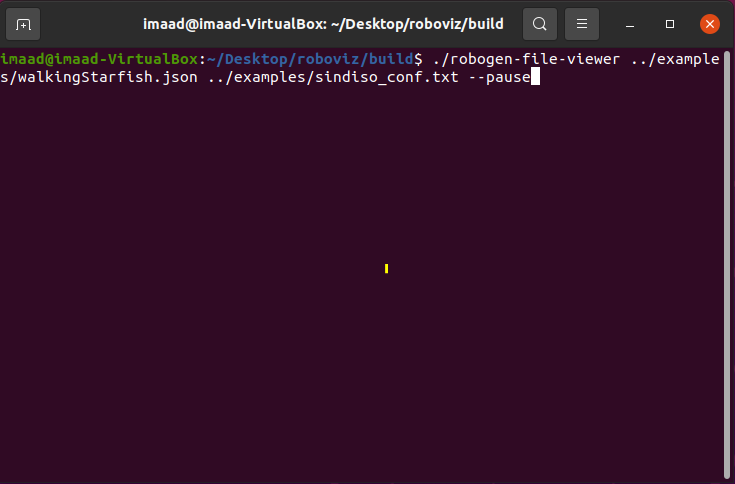
\includegraphics[width=0.8\textwidth]{run}
    \caption{commands in terminal }
    \label{fig:commands-in-terminal}
\end{figure}

Once entered, the screen shown in Figure \ref{fig:robots-in-visualiser} should
be displayed.
\begin{figure}[htpb]
    \centering
    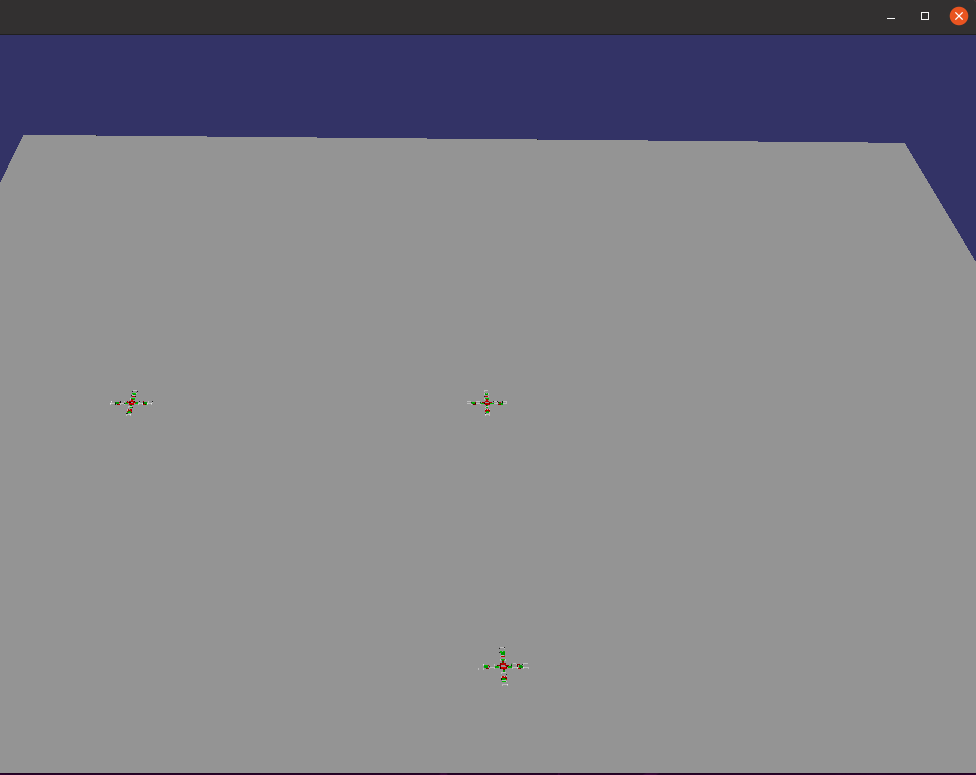
\includegraphics[width=0.8\textwidth]{visual1}
    \caption{Robots in Visualiser}
    \label{fig:robots-in-visualiser}
\end{figure}



\section{Full Test Runs}
What follows are the full, unabridged test runs. They can be executed manually
by building the project and then running the tests with ctest, like so:

\begin{verbatim}
    cd roboviz/build && rm -rf *
    cmake -DCMAKE_BUILD_TYPE=Release -G"Unix Makefiles" ../src
    time make -j2
    cp -r ../models ./
    ctest --verbose
\end{verbatim}


\label{s:full-test-runs}
\verbatiminput{TestRuns.txt}

\end{document}
